\documentclass[16.7pt]{jsarticle}

\usepackage{SPR}

\headerSPR
\begin{document}
	\titleSPR{\number\year}{\number\month}{\number\day}{D2}{吉田 皓太郎}
%%%%%%%%%%%%%%%%%%%%%%%%%%%%%%%%%%%%%%
	%\articleSPRabst
	%	\begin{itemize}
	%		\item =どういう事態か
	%	\end{itemize}
		
%今回のMTGの目的,何をディスカッションし,結果に何を得たいのかを決定する.※ミーティングごとに記入
	\articleSPRobj
		今回のMTGでは,D論の構成を現状までに達成された項目に基づき考察・再構築したものを記載しており,先生の意見を踏まえD論構成を確定させたいと考えている.また,そのD論構成に基づいた時,残りの少ない時間で何を行うべきかを議論し,今後の計画へと繋げたいと考えている.
		

%%%%%%%%%%%%%%%%%%%%%%%%%%%%%%%%%%%%%%
% 1.前回からのノルマ
	\articleSPRitemsone
		%\begin{enumerate}
		%	\item A
		%\end{enumerate}
		
		\tableofcontents
		
		
%%%%%%%%%%%%%%%%%%%%%%%%%%%%%%%%%%%%%%
%\begin{itemize}
%	\item 新規手法について
%	\item ISFAアウトライン
%\end{itemize}
%%%%%%%%%%%%%%%%%%%%%%%%%%%%%%%%%%%%%%
% 2.具体的な成果
	\articleSPRitemstwo
	\renewcommand{\labelitemi}{$\blacktriangledown$}
	%\renewcommand{\labelitemi}{$\bigcirc$}
	\newcommand{\argmax}{\mathop{\rm arg~max}\limits}
	\newcommand{\argmin}{\mathop{\rm arg~min}\limits}
	\newcommand{\Ker}{{\rm Ker}}
	\newcommand{\rank}{{\rm rank}}
%%%%%%%%%%%%%%%%%%%%%%%%%%%%%%%%%%%%%
	\section{【予備】局所修正法について}
		前回のMTGではそもそも計算の定義が間違っており,実行できませんでした.
		
		今までとそこまで解法の変わり映えしないという理由もあり,修正アルゴリズムを提案したいと考えております.このアルゴリズムでは,SCIで発表したように一度に変形させるのではなく,有限の修正操作を繰り返すことで点を満たすように移動することを考えたいと思います.
		
		それを踏まえて,一度今までの式を振り返ります.
		ある$ \varepsilon_c $および$ \bd{d} $に対して,修正後の長さ分布$ \varepsilon(s) $は,$ \bd{d} $が$ s $によって変化しない仮定の下で次式で表されます.
		\begin{equation}\label{eq:varDiffeq}
			\varepsilon' = -\frac{|u'\zetav_U\times \zetav_L|}{D \cos \alpha} \mathrm{sgn}((\zetav_L \times \zetav_U) \cdot \etav)\varepsilon := \sigma \varepsilon
		\end{equation}
		
		この式が$ s = s_c $で$ \varepsilon=\varepsilon_c $を取るならば,一意に
		\begin{equation}\label{eq:vareq}
			\varepsilon = \varepsilon_c \exp \left[ \int_{s_c}^{s} \sigma ds \right]
		\end{equation}
		と表されます.
		
		$ n $回目の操作の時の空間座標位置は$ \xv_{U,n} = \xv_U + \sum_{j=1}^{n} \varepsilon_i \bd{d}_i$と表され,この時,局所修正を想定するときには下記の要求を満たす必要があります.
		\begin{itemize}
			\item $ \int |\sum_{j=1}^{n} \varepsilon_j \bd{d}_j|^2 ds  $が最小であること
			\item $ \xv_{U,n}(s_c) = \bd{C} $であること
			\item $ \varepsilon $は$ s=s_c $で極値$ \varepsilon_c $をとる.
		\end{itemize}
		これを踏まえて,修正アルゴリズムを以下のように提案します.
		
		\begin{figure}[H]
			\centering
			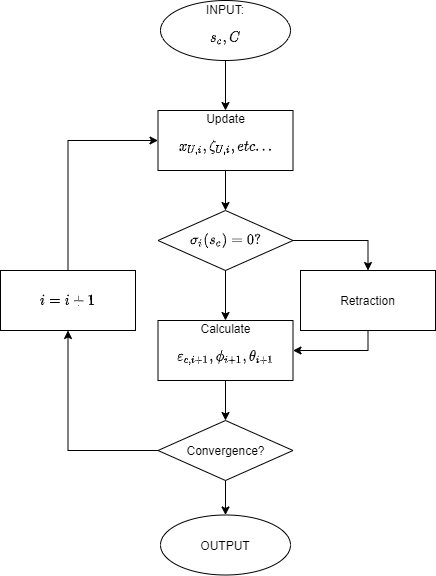
\includegraphics[width = 0.6\columnwidth]{figure/AmendFlow.png}
			\caption{A flow chart}
		\end{figure}
		
		順におって説明します.漸化式的に,$i$の情報から$ i+1 $の条件を求めます.
		まずはじめに,$ \sigma_i(s_c)=0 $を確認します.これは定義式から見れる通り,現在のステップ$ \bd{d}_{i+1} $に依存しません.そのため,$ s=s_c $が極値をとる条件であるとは限りません.(少なくとも初期値ではそう)この場合,レトラクションという定義する操作を行います.
		
		レトラクションという操作は次の条件を満たすように曲線を変形させます.はじめに,$ \sigma_i(s_p) =0$を満たす$ s_p $を求めます.次に,$ s=s_p $の時にある$ \varepsilon_{c,p} $だけ動かし,$ s=s_c $の時に極値をとるようにする.つまり,
		\begin{equation}\label{eq:CylinderEq}
			|\tilde{\zetav}_{U,i} \times \zetav_L| = 0
		\end{equation}
		ただし,チルダ記号は修正後であると定義しています.ここで,$ \bd{d}_p = \zetav_L(s_c) \cos \theta_p + \xiv_L(s_c) \sin \theta_p \cos \phi_p + \etav_L(s_c) \sin \theta \sin \phi_p $と表すと,式(\req{eq:CylinderEq})から次式を得ます.
		\begin{equation}\label{eq:CylinderEq2}
			(u'|\zetav_{U,i} \times \zetav_L|)^2 -2 (u'|\zetav_{U,i} \times \zetav_L|) \sigma_p \varepsilon_p \sin \theta \cos \phi + (\sigma_p \varepsilon_p \sin \theta)^2 =0
		\end{equation}
		この式が解を持つためには,$ \phi_p=0 $が必要であり,その時の$ \varepsilon_p $は次式で表されます.
		\begin{equation}\label{eq:vareps_p_eq}
			\varepsilon_{c,p} = \frac{D \cos \alpha}{\sin \theta \exp \left[ \int_{s_p}^{s_c} \sigma_i ds \right]}
		\end{equation}
		レトラクションにおいては,なるべく曲線を変形させたくないので,$ \varepsilon_{c,p} \rightarrow \min $を満たすと仮定することで,$ \theta_p = \frac{\pi}{2} $を得ます.これに従って,曲線を変形させます.この操作をレトラクションを定義しています.
		
		次に,$ s=s_c $で極値をとる仮定で話を進めます.$ \phi_{i+1},\theta_{i+1},\varepsilon_{c,i+1} $に従って曲線を変形させる時,局所修正の1番目の条件および,2番目の条件を$ |\xv_{U,n}(s_c) + \varepsilon_{i+1} \bd{d}_{i+1} - \bd{C}| \rightarrow \min$と解釈する.二つの条件は次式のように整理すれば,$ \varepsilon_{c,i+1} $に関して見れば二次関数であると捉えることができる.
		
		\begin{equation}\label{eq:No1_eq}
			\varepsilon_{c,i+1}^2 \int_{0}^{L} \exp \left[ \int_{s_c}^{s} 2\sigma_{i+1} (s) \right] + 2\varepsilon_{c,i+1} \bd{d}_{i+1} \cdot \left[\int_{0}^{L} \sum_{j=1}^{i} \varepsilon_j \bd{d}_j \exp \left[ \int_{s_c}^{s} 2\sigma_{i+1} (s) \right] \right] + \int_{0}^{L} |\sum_{j=1}^{i} \varepsilon_j \bd{d}_j|^2 ds
		\end{equation}
			
		\begin{equation}\label{eq:No2_eq}
			\varepsilon_{c,i+1}^2 -2 \varepsilon_{c,i+1} \bd{d}_{i+1} \cdot (\bd{C}-\xv_{U,n}) + |\bd{C}-\xv_{U,n}|^2
		\end{equation}
		
		この二つの最小値条件は,$ \varepsilon_{c,i+1} $が一致することから次式で表現される.
		\begin{equation}\label{eq:var_c_eq}
			-\frac{\bd{d}_{i+1} \cdot \int_{0}^{L} \sum_{j=1}^{i} \varepsilon_j \bd{d}_j  \exp \left[ \int_{s_c}^{s} 2\sigma_{i+1} (s) \right]}{\int_{0}^{L} \exp \left[ \int_{s_c}^{s} 2\sigma_{i+1} (s) \right]} = \bd{d}_{i+1} \cdot (\bd{C}-\xv_{U,n})
		\end{equation}
		
		のちの計算で使用するため,次式のように制約式として表現する.
		\begin{equation}\label{eq:var_c_eq2}
			\bd{d}_{i+1} \cdot \left( \frac{\int_{0}^{L} \sum_{j=1}^{i} \varepsilon_j \bd{d}_j \exp \left[ \int_{s_c}^{s} 2\sigma_{i+1} (s) \right]}{\int_{0}^{L} \exp \left[ \int_{s_c}^{s} 2\sigma_{i+1} (s) \right]} + (\bd{C}-\xv_{U,n}) \right) := \bd{d}_{i+1} \cdot \bd{\mu} = 0
		\end{equation}
		さらに,$ \bd{d}_{i+1} $は$ \bd{C}-\xv_{U,n} $の方向になるべく平行となる方が解にたどり着ける可能性が高いため,$  \bd{d}_{i+1} \cdot \bd{C}-\xv_{U,n} \rightarrow \max$が要求される.式(\ref{eq:var_c_eq2})より,$ \bd{\mu} $を表すオイラー角を$ \phi_q, \theta_q $とおけば,$ \bd{d}_{i+1} $は$ \theta_q, \phi_q$および任意の角度$ \psi $を用いて表すことができ,これを用いて$ \bd{d}_{i+1} \cdot (\bd{C}-\xv_{U,n}) $の極値条件を求めれば,解を得ることができると思われる.
	\subsection{RenewRetraction}
		母線の分布に沿って曲線を操作するときには,どのような$ \varepsilon $の分布を選んでも,可展面の式を満たすことができることを証明する.接平面式を求めると,
		\begin{equation}\label{eq:TanEq_withGene}
			\left\{ (u'\zetav_U + \varepsilon' \bd{d}_2 + \varepsilon \bd{d}_2') \times \zetav_L \right\}\cdot(D+\varepsilon)\bd{d}_2 = 0
		\end{equation}
		となる.計算過程では,$ \xv_U - \xv_L = D \bd{d}_2 $であることを用いている.スカラー3重積の変換操作をいくつか行うことで,
		\begin{equation}\label{eq:TanEq_ver2}
			(\zetav_L \times \bd{d}_2 )\cdot (u'\zetav_U + \varepsilon' \bd{d}_2 + \varepsilon \bd{d}_2') = 0
		\end{equation}
		と変換することができる.ここで操作前は可展面であることから,$ \zetav_U $は接平面上に存在しており,$ \bd{d}_2' = -(\alpha' + \omega_{\eta}) \bd{d}_1 $と計算できることから,この式は恒等式となる.以上より,題意は示された.
		
		このことから,母線方向であれば任意の$ \varepsilon $分布を設定し変形操作を行うことができる.ただし,可展面の情報は変化しないことから,自己交差を起こすかどうかは常に注意しなければならない.
		$ \varepsilon = \bd{a} \cdot \bd{e}$のように,基底関数の線形和で表記する.局所変形性を考慮することから,$ \varepsilon $は
		\begin{equation}\label{eq:min_vareps}
			\min \int_{0}^{L} \varepsilon^2 ds
		\end{equation}
		を満たす.また,制約条件として次式らを与える.
		\begin{eqnarray}
			\varepsilon' \cos \alpha -(\alpha'+\omega_{\eta})\sin \alpha - u' (\zetav_U \times \zetav_L) \cdot \etav_L &=& 0 \\
			\varepsilon - \bd{d}_2 \cdot (\bd{C} - \bd{x}_U) &=& 0
		\end{eqnarray}
		これらはそれぞれ,のちに用いるための極値条件を与える式および,最大限の移動量を確保するための式である.この最適化問題を解けば最適な分布を得ることができると想定される.
		
		この最適化問題をラグランジュ乗数を用いて次のように表す.
		\begin{eqnarray}\label{eq:LagrangeEq}
			L(\bd{a}) &=&  \int_{0}^{L} \varepsilon^2 ds - \lambda_1(\varepsilon' \cos \alpha -(\alpha'+\omega_{\eta})\sin \alpha - u' (\zetav_U \times \zetav_L) \cdot \etav_L) - \lambda_2 (\varepsilon - \bd{d}_2 \cdot (\bd{C} - \bd{x}_U)) \\
			&:= & \bd{a}^T \bd{M} \bd{a} - \lambda_1(\bd{a} \bd{C}_1 - p_1) -\lambda_2(\bd{a} \bd{C}_2 - p_2) 
		\end{eqnarray}
		KKT条件から$ \bd{a} $は
		\begin{equation}\label{eq:Calc_Coef}
			\bd{a} = \lambda_1 \bd{C}_1^T \bd{M}^{-1} + \lambda_2 \bd{C}_2^T \bd{M}^{-1} 
		\end{equation}
		と表すことができる.また,KKT条件の式から,
		\begin{eqnarray}
			\lambda_1 \bd{C}_1^T \bd{M}^{-1} \bd{C}_1 + \lambda_2 \bd{C}_2^T \bd{M}^{-1} \bd{C}_1  &=& p_1 \\
			\lambda_1 \bd{C}_1^T \bd{M}^{-1} \bd{C}_2 + \lambda_2 \bd{C}_2^T \bd{M}^{-1} \bd{C}_2 &=& p_2
		\end{eqnarray}
		を得る.この2つを連立して解くことで,$ \bd{a} $を得る.
		これを操作の代わりに置く.
	\section{【メモ用】オイラー角表記}
	\begin{equation}
		\left[ \begin{array}{ccc}
			\cos \theta \cos \psi & -\cos \theta \sin \psi & \sin \theta \\
			\cos \phi \sin \psi + \sin \phi \sin \theta \cos \psi & \cos \phi \cos \psi - \sin \phi \sin \theta \sin \psi & -\sin \phi \cos \theta \\
			\sin \phi \sin \psi - \cos \phi \sin \theta \cos \psi & \sin \phi \cos \psi + \cos \phi \sin \theta \sin \psi & \cos \phi \cos \theta
		\end{array}\right]
	\end{equation}	
		
		
	\section{次回のMTGについて(終了後記載)}
	\begin{itemize}
		\item  
		\item 
	\end{itemize}
	###
	\newpage
%\vspace{10cm}
%%%%%%%%%%%%%%%%%%%%%%%%%%%%%%%%%%%%%%
% 3.達成できなかったこととその問題点
	%\articleSPRthree
	
%%%%%%%%%%%%%%%%%%%%%%%%%%%%%%%%%%%%%%

%\vspace{14cm}
%%%%%%%%%%%%%%%%%%%%%%%%%%%%%%%%%%%%%%
	%\articleSPRfour
	%\articleSPRfive
\end{document}
